%%%%%%%%%%%%%%%%%%%%%%%%%%%%%%%%%%%%%%%%%%%%%%%%%%%%%%%%%%%%%%
% --> INTRODUCCIÓN
%%%%%%%%%%%%%%%%%%%%%%%%%%%%%%%%%%%%%%%%%%%%%%%%%%%%%%%%%%%%%%
\section{Introducción}

Como se menciona en \cite{R3}, en ciencias de la computación, un árbol binario es una estructura de datos en la cual cada nodo puede tener un hijo izquierdo y un hijo derecho. No pueden tener más de dos hijos (de ahí el nombre "binario"). Si algún hijo tiene como referencia a null, es decir que no almacena ningún dato, entonces este es llamado un nodo externo. En el caso contrario el hijo es llamado un nodo interno. Usos comunes de los árboles binarios son los árboles binarios de búsqueda, los montículos binarios y Codificación de Huffman.

En la figura \ref{fig:tree}, se observa una imagen que ayuda a ejemplificar la estructura básica de un árbol binario.

\begin{figure}[H]
\centering
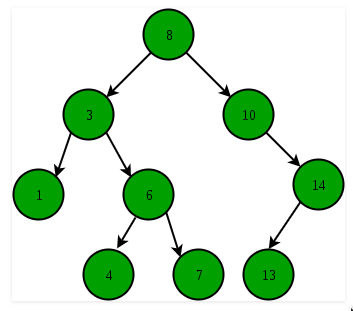
\includegraphics[width=0.45\textwidth]{imgs/Labo9/tree.png}
\caption{Estructura de datos tipo árbol}
\label{fig:tree}
\end{figure}

Un árbol binario es un árbol en el que ningún nodo puede tener más de dos subárboles. En un árbol binario cada nodo puede tener cero, uno o dos hijos (subárboles). Se conoce el nodo de la izquierda como hijo izquierdo y el nodo de la derecha como hijo derecho. Además se debe cumplir que ningún valor del árbol se puede repetir y además, el hijo de la izquierda es menor y el hijo de la derecha es mayor.

Existen tipos de árboles binarios que suelen usarse para fines específicos, como:

\begin{itemize}
    \item Árbol binario de búsqueda
    \item Árbol de Fibonacci
\end{itemize}

También es común hablar de métodos de recorrido de un árbol binario, por lo que más comunes son:

\begin{itemize}
    \item Recorrido en \texttt{preorden}
    \item Recorrido en \texttt{postorden}
    \item Recorrido en \texttt{inorden}
\end{itemize}

Por lo tanto, en este laboratorio se va a trabajar con este tipo de estructura de datos.




%%%%%%%%%%%%%%%%%%%%%%%%%%%%%%%%%%%%%%%%%%%%%%%%%%%%%%%%%%%%%%
% --> OBJETIVOS
%%%%%%%%%%%%%%%%%%%%%%%%%%%%%%%%%%%%%%%%%%%%%%%%%%%%%%%%%%%%%%
\subsection{Objetivos}

%%%%%%%%%%%%%%%%%%%%%%%%%%%%%%%%%%%%%%%%%%%%%%%%%%%%%%%%%%%%%%
% --> OBJETIVO GENERAL
%%%%%%%%%%%%%%%%%%%%%%%%%%%%%%%%%%%%%%%%%%%%%%%%%%%%%%%%%%%%%%
\subsubsection{Objetivo General}
\begin{itemize}
\item Desarrollar una estructura de datos tipo árbol binario. 
\end{itemize}

%%%%%%%%%%%%%%%%%%%%%%%%%%%%%%%%%%%%%%%%%%%%%%%%%%%%%%%%%%%%%%
% --> OBJETIVOS ESPECÍFICOS
%%%%%%%%%%%%%%%%%%%%%%%%%%%%%%%%%%%%%%%%%%%%%%%%%%%%%%%%%%%%%%
\subsubsection{Objetivos Específicos}
\begin{itemize}
\item Realizar las funciones para la insertar y remover nodos de un árbol binario y poder realizar operaciones básicas.
\item Crear algoritmos de recorrido de árboles binarios.
\item Programar el algoritmo de balanceo de un árbol.
\item Validar los códigos desarrollados con una serie de pruebas en el programa principal.
\end{itemize}

%%%%%%%%%%%%%%%%%%%%%%%%%%%%%%%%%%%%%%%%%%%%%%%%%%%%%%%%%%%%%%
% --> ENUNCIADO
%%%%%%%%%%%%%%%%%%%%%%%%%%%%%%%%%%%%%%%%%%%%%%%%%%%%%%%%%%%%%%
%\newpage
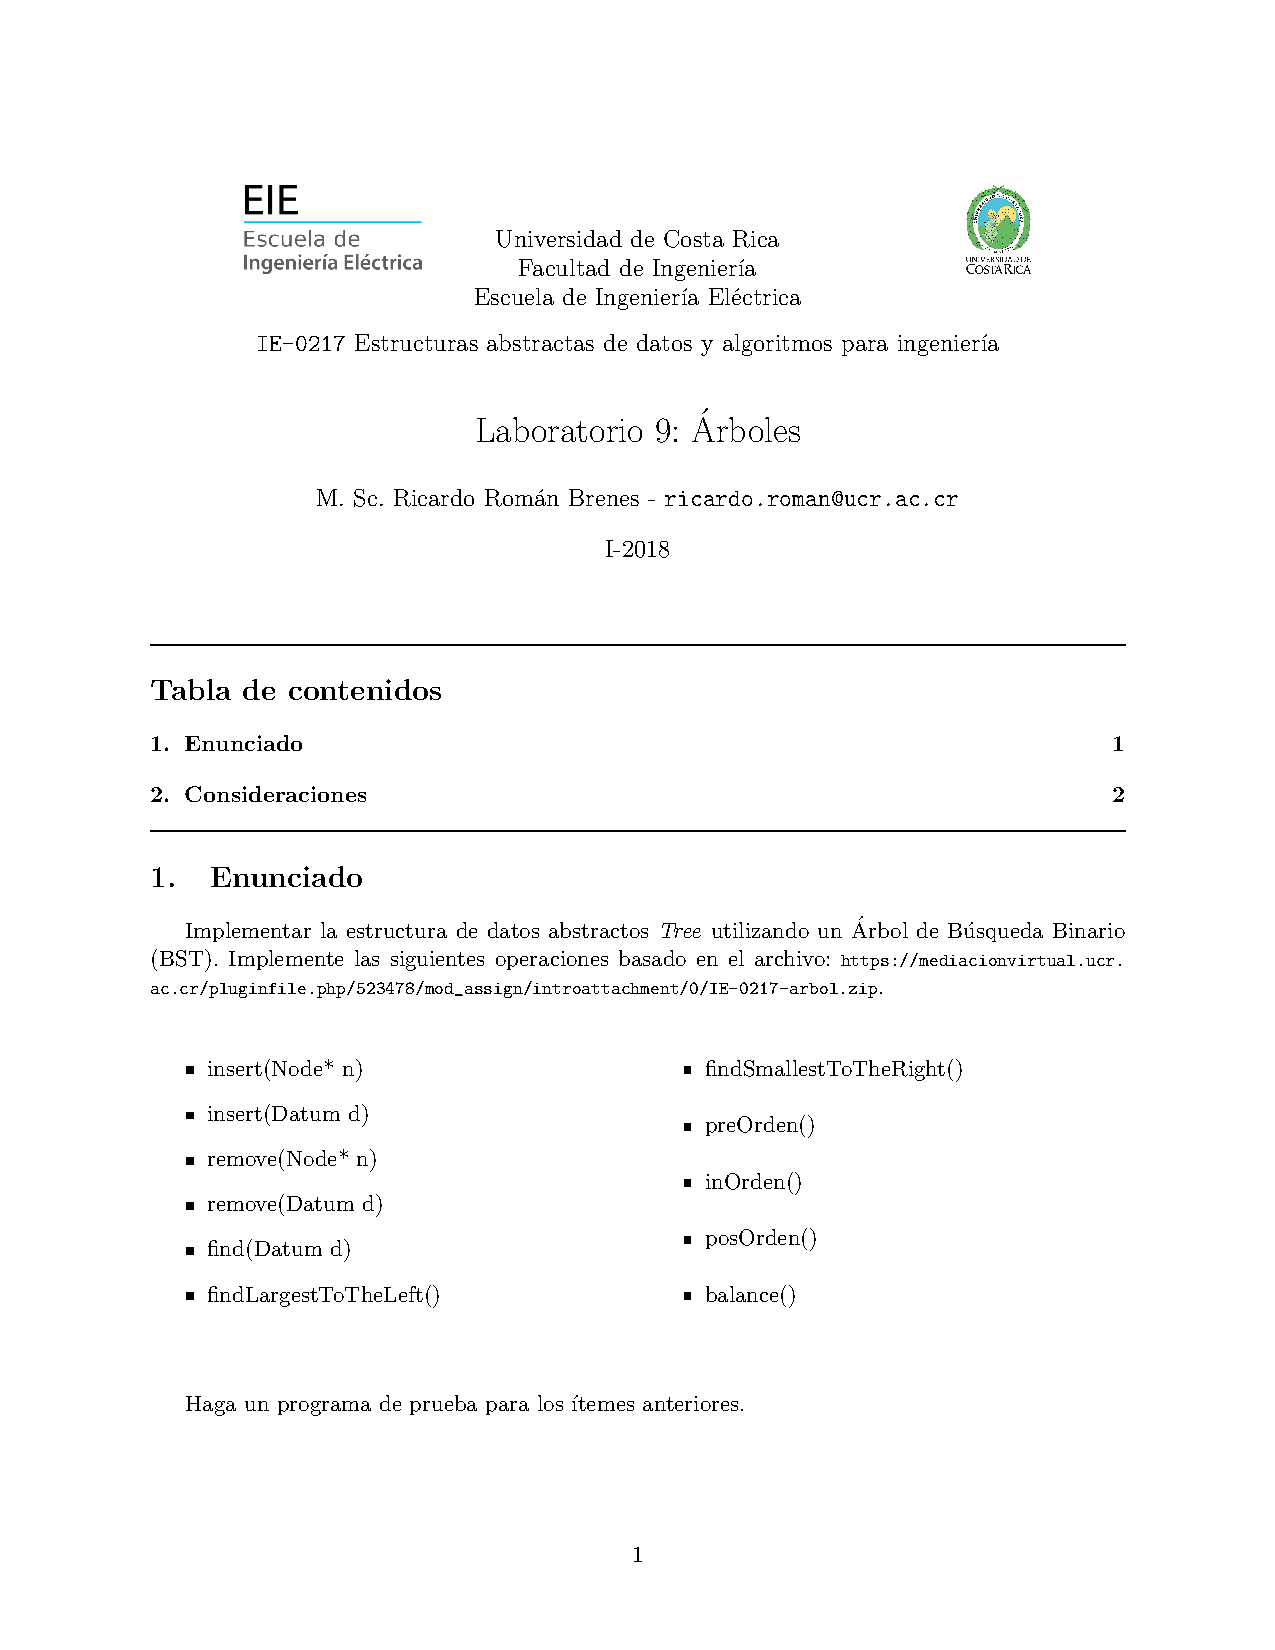
\includepdf[pages=1,pagecommand=\section{Enunciado}, scale=0.8]{enunciados/enun9} 
\includepdf[pages=2,pagecommand={},scale=0.8]{enunciados/enun9}

%%%%%%%%%%%%%%%%%%%%%%%%%%%%%%%%%%%%%%%%%%%%%%%%%%%%%%%%%%%%%%
% --> SOLUCIÓN
%%%%%%%%%%%%%%%%%%%%%%%%%%%%%%%%%%%%%%%%%%%%%%%%%%%%%%%%%%%%%%
\section{Solución}
Para la resolución del laboratorio se utilizaron los archivos proporcionados por el profesor y se procedió a la creación de una serie de métodos para operar sobre el árbol de búsqueda binaria, estos métodos se explican a continuación.
\subsection{Métodos implementados:}

\begin{itemize}
    \item \texttt{insert(Node* n)}: Esta función inserta un nodo \texttt{n} en el árbol, y lo acomoda en la posición adecuada. Para su implementación fue necesario utilizar el método \texttt{iterativeInsert(Node* n)} al que se le agregaron una serie de líneas para almacenar los datos de los hijos derechos e izquierdos.
    
    \begin{minted}[linenos,autogobble,bgcolor=bg,breaklines,fontsize=\footnotesize ]{c++}
    
    void insert(Node* n)
    {
      cout << "Inserting new node "<< n->getDatum() << endl;
      this->nodes++;
      if (!this->root) this->root = n;
      else iterativeInsert(n);
    }
    
    void iterativeInsert(Node* n) 
    {
      bool end = false;
      Node* current = this->root;
      Node* temp;
      while (!end)
      {
        if (!current)
        {
          cout<<"bug:"<< (void*)temp<< endl;
          n->setAncestor(temp);
          current = n;
          end = true;
        } else
        {
          if (current->getDatum() < n->getDatum())
          {
            temp = current;
            current = current->getRightChild();
          }
          else
          {
            temp = current;
            current = current->getLeftChild();
          }
        }
      }
      temp = current->getAncestor();
      if(n->getDatum()<temp->getDatum())
        temp->setLeftChild(n);
      else
        temp->setRightChild(n);
    }
    
    \end{minted}
    
    \item \texttt{remove(Node* n)}: El método \texttt{remove} elimina un nodo del árbol y libera la memoria de los punteros utilizados. Fue necesario implementar otro método que funciona en conjunto llamado \texttt{deleteNode(Node* n, Datum key)} y es llamado desde la función remover.
    
    \begin{minted}[linenos,autogobble,bgcolor=bg,breaklines,fontsize=\footnotesize ]{c++}
    
    void remove(Node* n)
    {
      cout << "Deleting node "<< n->getDatum() << endl;
      this->nodes--;
      this->root = deleteNode(this->root,n->getDatum());
    }
    
    Node* deleteNode(Node* n, Datum key)
    {
      if (key < n->getDatum())
          n->setLeftChild(deleteNode(n->getLeftChild(), key));

      else if (key > n->getDatum())
          n->setRightChild(deleteNode(n->getRightChild(), key));

      else
      {
          if (n->getLeftChild() == NULL)
          {
              Node *temp = n->getRightChild();
              delete n;
              return temp;
          }
          else if (n->getRightChild() == NULL)
          {
              Node *temp = n->getLeftChild();
              delete n;
              return temp;
          }

          Node* temp = findSmallestToTheRight(n);

          n->setDatum(temp->getDatum());

          n->setRightChild(deleteNode(n->getRightChild(), temp->getDatum()));
      }
      return n;
    };
    \end{minted}

    \item \texttt{find(Datum d)}: Este método es el encargado de devolver la dirección en la que se encuentra el dato \texttt{d}, para esto utiliza una función \texttt{search(Node* n, Datum d)} que comprueba si el dato se encuentra en el árbol.
    
    \begin{minted}[linenos,autogobble,bgcolor=bg,breaklines,fontsize=\footnotesize ]{c++}
    
    Node* find(Datum d)
    {
      return search(this->root,d);
    }

    Node* search(Node* n, Datum d)
    {
      if (n == 0x0) {cout<<"Data '"<<d<< "' hasn't been found in the tree"<<endl; return 0x0;}
      else if (n->getDatum() == d) return n;

      if (n->getDatum() < d) return search(n->getRightChild(), d);

      return search(n->getLeftChild(), d);
    }

    Datum find(Node* n)
    {
      return n->getDatum();
    }

    \end{minted}

    \item \texttt{findLargestToTheLeft()}: Como lo dice su nombre, esta función retorna el nodo más grande a la izquierda del árbol.
    
    \begin{minted}[linenos,autogobble,bgcolor=bg,breaklines,fontsize=\footnotesize ]{c++}
    
    Node* findLargestToTheLeft(Node* n)
    {
        Node* s = n->getLeftChild();
        if (s == NULL){
          cout << "No hay elementos a la izquierda" << endl;
          return s;
        }
        while (s->getRightChild()!= NULL)
          s = s->getRightChild();
        return s;
    }
    \end{minted}

    \item \texttt{findSmallestToTheRight()}: Función que regresa el nodo más pequeño a la derecha del árbol.
    
    \begin{minted}[linenos,autogobble,bgcolor=bg,breaklines,fontsize=\footnotesize ]{c++}
    Node* findSmallestToTheRight(Node* n)
    {
      Node* s = n->getRightChild();
      if(s == NULL) {cout << "No hay elementos a la derecha" << endl; return s;}
      while(s->getLeftChild() != NULL)
        s = s->getLeftChild();
      return s;
    }
    \end{minted}
    
    \item \texttt{Funciones de ordenamiento}: Para el ordenamiento de los elementos del árbol se implementaron tres métodos con tres tipos diferentes de ordenamiento. La función \texttt{preOrden()} ordena los elementos del árbol en orden ascendente, mientras que la función \texttt{posOrden()} lo hace al contrario, es decir, descendentemente. La última forma de ordenamiento, \texttt{inOrden()}, es peculiar debido a que coloca primero el valor de la raíz del árbol, seguido por los valores menores, y a continuación todos los valores mayores. Todos estos métodos funcionan recibiendo como parámetro el nodo raíz del árbol.
    
    \begin{minted}[linenos,autogobble,bgcolor=bg,breaklines,fontsize=\footnotesize ]{c++}
    void preOrden(Node * n)
    {
      if (n == NULL) return;
      preOrden(n->getLeftChild());
      cout << n->getDatum() << endl;
      preOrden(n->getRightChild());
    };

    void posOrden(Node * n)
    {
      if (n == NULL ) return;
      posOrden(n->getRightChild());
      cout << n->getDatum() << endl;
      posOrden(n->getLeftChild());
    };

    void inOrden(Node * n)
    {
      if (n == NULL) return;
      cout << n->getDatum() << endl;
      inOrden(n->getLeftChild());
      inOrden(n->getRightChild());
    };

    \end{minted}
    
    \item \texttt{balance()}: Se buscó implementar un método para balancear un árbol binario. Es decir, que dado un árbol que tiene una cantidad mayor de niveles que la necesaria, se modifique de tal forma que se use la menor cantidad de niveles posible y que las ramas estén distribuidas equitativamente. Para lograr esto, se decidió almacenar todos los valores de los nodos del árbol, en orden ascendente (\textit{inOrder}) en una lista enlazada (en este caso, se utilizó la clase \texttt{listWithPointer} anteriormente creada). Luego de esto, se quiso implementar un algoritmo que, partiera la lista a la mitad y tomara este valor medio para insertarlo en el árbol. Haciendo esto recursivamente, se lograría insertar los nodos en el orden óptimo de tal forma que el árbol quedara balanceado. Este último paso no se logró implementar satisfactoriamente.
    
    \begin{minted}[linenos,autogobble,bgcolor=bg,breaklines,fontsize=\footnotesize ]{c++}
    void balancear()
    {
	    if (this->getRootNode() == NULL) cout << "No se puede balancear arbol vacío" << endl;
		fillArray(this->root);
		//vaciar el árbol
		cout << "destruyendo" << endl;
		DestroyRecursive(this->root);
		//reconstruir árbol a partir de elementos de la lista
		ListToBST(this->list->getFirst(),0,this->list->getSize()-1);
    // };
    
    //funcion para pasar elementos del arbol a una lista enlazada
    void fillArray(Node * n) // l d r
    {
    if (n == NULL) return;
    fillArray(n->getLeftChild());
    this->list->insert(n->getDatum());
    fillArray(n->getRightChild());
    };
    
    void ListToBST(SimpleNode<Datum>* element, int start, int end){
		if (start>end) return;
		int mid = start + (end-start)/2;
		cout << "mid: " << mid << endl;
		Node* leftChild = listToBST(element,start,mid-1);
		cout << "created lc" << endl;
		cout << "element value: " << element->value << endl;
		Node* parent = new Node(element->value);
		cout << "created node" << endl;		parent->setLeftChild(leftChild);
		element=element->getNext();
		parent->setRightChild(listToBST(element,mid,end));
		this->insert(parent);
	};
    \end{minted}
    
\end{itemize}


%%%%%%%%%%%%%%%%%%%%%%%%%%%%%%%%%%%%%%%%%%%%%%%%%%%%%%%%%%%%%%
% --> RESULTADOS
%%%%%%%%%%%%%%%%%%%%%%%%%%%%%%%%%%%%%%%%%%%%%%%%%%%%%%%%%%%%%%
\section{Resultados}

En las siguientes figuras se observan los resultados al ejecutar las funciones creadas, para esto se utilizó el código escrito en el \texttt{main}, que se adjunta a continuación. En la Figura \ref{fig:1} se observa la creación de un árbol y además se observa que se le añaden nodos con diversos valores. EN la parte inferior se puede observar el resultado de imprimir el árbol, donde se nota la correspondencia de los punteros de los nodos, lo que nos indica que estos están correctamente enlazados, este árbol tiene una estructura como la que se observa entre las líneas 13 y 20 del código.


    
    \begin{minted}[linenos,autogobble,bgcolor=bg,breaklines,fontsize=\footnotesize ]{c++}
    #include <iostream>
    #include "../include/BST.hpp"
    #include "../include/BSTNode.hpp"
    using namespace std;
    
    int main(int argc, char** argv)
    {
        //Se crea un árbol binario
        BST< BSTNode<int>,int >* littleTree = new BST< BSTNode<int>,int >();
        //Se crean nodos para el árbol
        BSTNode<int>* _50 = new BSTNode<int>(0x0, 0x0, 50);
        BSTNode<int>* _25 = new BSTNode<int>(0x0, 0x0, 25);
        BSTNode<int>* _75 = new BSTNode<int>(0x0, 0x0, 75);
        BSTNode<int>* _10 = new BSTNode<int>(0x0, 0x0, 10);
        BSTNode<int>* _420 = new BSTNode<int>(0x0, 0x0, 420);
        BSTNode<int>* _60 = new BSTNode<int>(0x0, 0x0, 60);
        BSTNode<int>* _40 = new BSTNode<int>(0x0, 0x0, 40);
        BSTNode<int>* _15 = new BSTNode<int>(0x0, 0x0, 15);
        /* Insertando los nodos al árbol, para que quede de la siguiente manera:
        *                    50
        *                  /    \
        *                25     75
        *               /  \   /  \
        *             10  40  60  420
        *               \
        *               15
        */
        littleTree->insert(_50);
        littleTree->insert(_25);
        littleTree->insert(_75);
        littleTree->insert(_10);
        littleTree->insert(_420);
        littleTree->insert(_60);
        littleTree->insert(_40);
        littleTree->insert(_15);
        // Imprimiendo árbol manualmente nodo por nodo
        cout <<endl<<separator<<"Printing resulting tree" <<endl<<endl;
        _50->printMe();
        _25->printMe();
        _10->printMe();
        _75->printMe();
        _420->printMe();
        _60->printMe();
        _40->printMe();
        _15->printMe();
    \end{minted}



\begin{figure}[H]
\centering
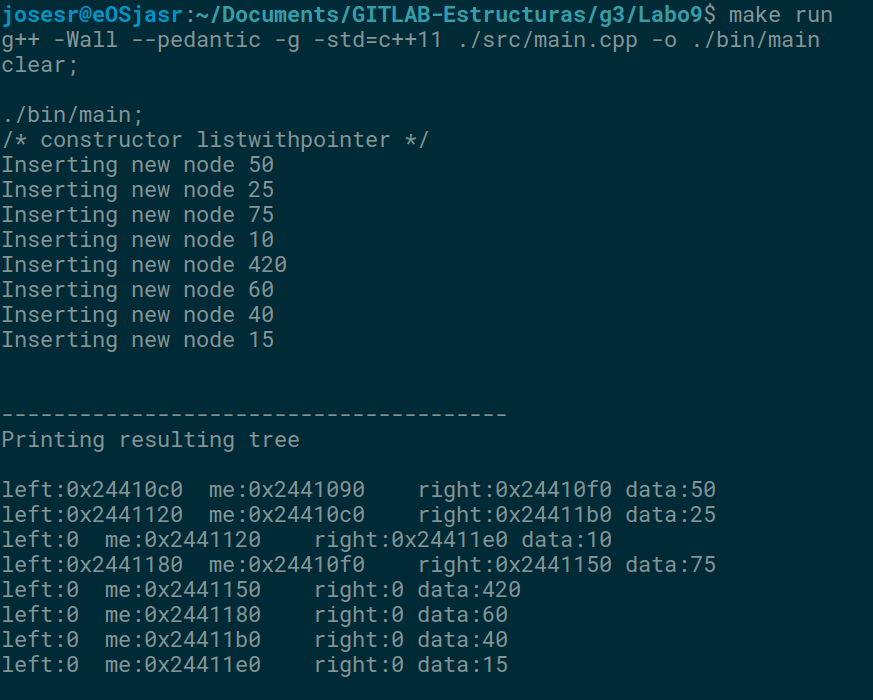
\includegraphics[width=\textwidth]{imgs/Labo9/L9-1.png}
\caption{Creación del árbol, inserción de nodos e impresión del árbol.}
\label{fig:1}
\end{figure}

En la Figura \ref{fig:2} se puede observar las pruebas realizadas para el despliegue de ciertos datos de interés, por ejemplo, podemos observar la raíz del árbol que se creó anteriormente, así como el valor que este nodo almacena. También se probaron las funciones \texttt{findLargestToTheLeft} y \texttt{findSmallestToTheRight}, que devolvieron los valores esperados. Además se comprobó el correcto funcionamiento de las funciones de búsqueda \texttt{find}.

\begin{minted}[linenos,autogobble,bgcolor=bg,breaklines,fontsize=\footnotesize ]{c++}
    const char * separator = "\n---------------------------------------\n"
    cout <<endl<<separator<<"----------- Algunas pruebas ----------- " << endl<<endl;
    BSTNode<int>* littleRoot = littleTree->getRootNode();
    cout << "Root del árbol: " << littleRoot << endl;
    cout << "Valor almacenado en el root: " << littleTree->getRootValue() << endl;
    BSTNode<int>* test = new BSTNode<int>(0);
    cout <<separator<< "Probando findLargestToTheLeft: " << endl;
    test = littleTree->findLargestToTheLeft(littleRoot);
    test->printMe();
    cout << endl << "Probando findSmallestToTheRight: " << endl;
    test = littleTree->findSmallestToTheRight(littleRoot);
    test->printMe();
    cout <<separator<< "Probando find(-2) (dato que no existe): " << endl;
    test = littleTree->find(-2);
    test->printMe();
    cout << endl << "Probando find(root): " << endl;
    cout << littleTree->find(littleRoot) << endl;
    cout << endl <<  "Probando find(root->leftChild): " << endl;
    cout << littleTree->find(littleRoot->getLeftChild()) << endl;
    cout << endl << "Probando find(root->rightChild): " << endl;
    cout << littleTree->find(littleRoot->getRightChild()) << endl;
\end{minted}

\begin{figure}[H]
\centering
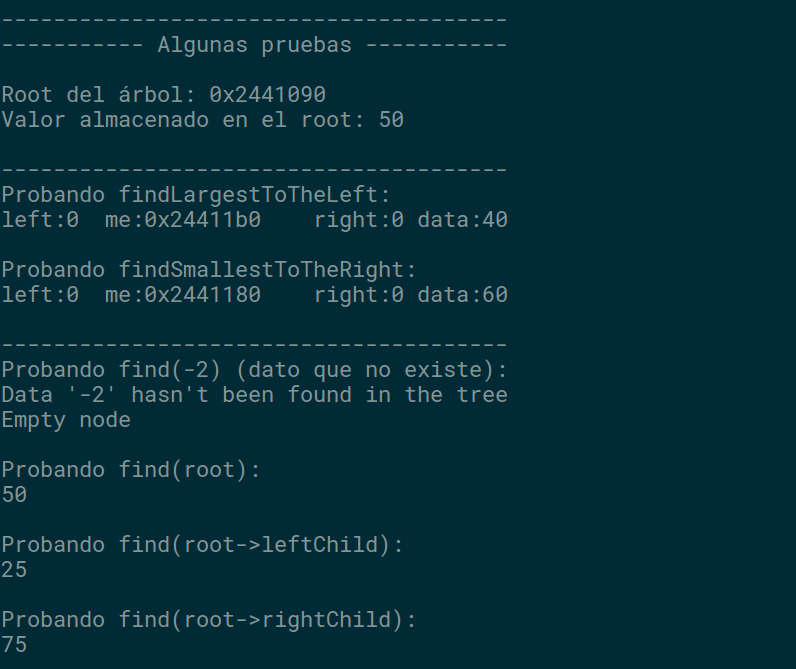
\includegraphics[width=0.85\textwidth]{imgs/Labo9/L9-2.png}
\caption{Prueba de métodos de búsqueda.}
\label{fig:2}
\end{figure}



\begin{minted}[linenos,autogobble,bgcolor=bg,breaklines,fontsize=\footnotesize ]{c++}
    cout <<separator<<"Imprimiendo preOrden " << endl<<endl;
    littleTree->preOrden(littleRoot);
    cout <<separator<<"Imprimiendo  inOrden " << endl<<endl;
    littleTree->inOrden(littleRoot);
    cout <<separator<<"Imprimiendo  posOrden " << endl<<endl;
    littleTree->posOrden(littleRoot);
    \end{minted}

Al aplicar los tres tipos de ordenamiento se obtiene el resultado de la Figura \ref{fig:3}, donde se observa que son resultados satisfactorios.

\begin{figure}[H]
\centering
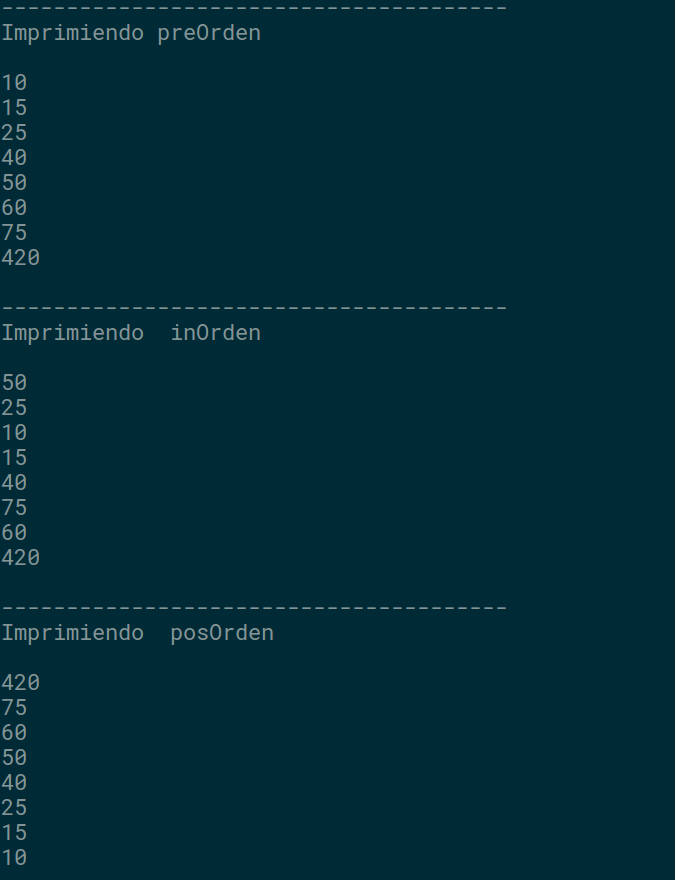
\includegraphics[width=0.8\textwidth]{imgs/Labo9/L9-3.png}
\caption{Impresión de los métodos de ordenamiento.}
\label{fig:3}
\end{figure}


\begin{minted}[linenos,autogobble,bgcolor=bg,breaklines,fontsize=\footnotesize ]{c++}
    cout <<separator<<"Cantidad de niveles:" << endl<<endl;
    cout << littleTree->getLevels() << endl;
    cout << separator << "Borrando el nodo 50" << endl;
    littleTree->remove(_50);
    cout << "Nuevo root del árbol: " << littleTree->getRootNode() << endl;
    cout << "Valor del nuevo root: " << littleTree->getRootValue() << endl;
    littleRoot = littleTree->getRootNode();
    /*                  60
    *                  /  \
    *                 25  75
    *                /  \   \
    *               10  40  420
    *                 \
    *                 15
    */
    cout << separator << "Llenar lista con valores almacenados, en orden ascendente: " << endl;
    littleTree->fillArray(littleRoot);
    littleTree->printList();
    cout <<endl<<"test----- " << endl<<endl
    littleTree->remove(_40);
    cout << "Root value: " << littleTree->getRootValue() << endl;
    \end{minted}

En la Figura \ref{fig:4} se imprimió la cantidad de niveles del árbol obtenida con el método creado y ya comentado. También se probó la eliminación del nodo raíz del árbol y seguidamente la asignación de una nueva raíz. Con el método \texttt{fillArray} se creó una lista enlazada que contiene los valores del árbol ordenados de forma ascendente.

\begin{figure}[H]
\centering
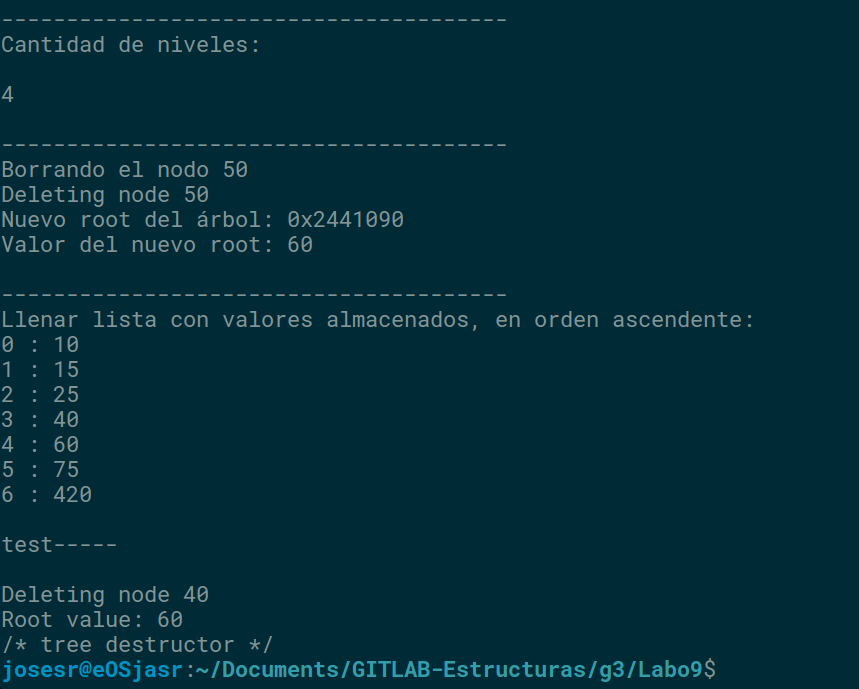
\includegraphics[width=0.9\textwidth]{imgs/Labo9/L9-4.png}
\caption{Creación de una lista con los valores ordenados del árbol.}
\label{fig:4}
\end{figure}


%%%%%%%%%%%%%%%%%%%%%%%%%%%%%%%%%%%%%%%%%%%%%%%%%%%%%%%%%%%%%%
% --> CONCLUSIONES
%%%%%%%%%%%%%%%%%%%%%%%%%%%%%%%%%%%%%%%%%%%%%%%%%%%%%%%%%%%%%%
\section{Conclusiones}


Como conclusiones se tiene que:

\begin{itemize}
\item Se implementó correctamente una estructura de datos de tipo árbol binario.
\item Se logró  implementar correctamente las funciones para insertar y remover nodos en un árbol binario.
\item Se crearon correctamente los métodos necesarios para recorrer los árboles, así como para ordenar sus elementos.
\item La creación del método de balanceo del árbol resultó satisfactoria y eficaz.
\item Se comprobó el funcionamiento de todos los métodos con una serie de pruebas desplegadas en la terminal.
\end{itemize}


%%%%%%%%%%%%%%%%%%%%%%%%%%%%%%%%%%%%%%%%%%%%%%%%%%%%%%%%%%%%%%
% --> BIBLIOGRAFIA
%%%%%%%%%%%%%%%%%%%%%%%%%%%%%%%%%%%%%%%%%%%%%%%%%%%%%%%%%%%%%%
\begin{thebibliography}{IEEE}
\bibitem{R1} Talens, S. \textbf{\textit{Curso de programación en C++}}. EUI (UPV) Valencia, 17 al 28 de Julio de 1995. 

\bibitem{R2} Raffo, E. \textbf{\textit{Programación genérica en C++, usando Metaprogramación}}. 2007. Sistemas de Informática. 

\bibitem{R3} Wikipedia \textbf{\textit{Árbol Binario}}. Tomado el 20 de Junio del 2018 en: \url{https://es.wikipedia.org/wiki/\%C3\%81rbol_binario}.

\end{thebibliography}